\chapter{Introduction}
\label{chapter:intro}

\subsection{Research Motivation}

The survival of enterprises is more and more dependant on the way they collect, use and share data. With the development of information and communication technology, sharing data between supply chains has improved the competitive advantages of all of the parties. However, there still exists a lack of information that would allow companies to better develop their products, coordinate actions and serve their customers. This information is most often held by another enterprise, possibly in another supply chain, who is not willing to share it due to losing some of the companys competitive advantage. Balancing between competition and cooperation - coopetition - is becoming an increasing trend within the industry and academica \cite{}. This study aims to identify the factors that prevent and support sharing data between enterprises, in an attempt to create an environment most suitable for sharing data and thus improving organizational efficiency.

The role of knowledge as a vital enabler for competitive differentiation has been emphasized since Penrose, 1995 \cite{penrose1995theory}. Knowledge sharing processes across organizational boundaries have recently been investigated by multiple academics \cite{loebbecke2016managing, chiu2006understanding, loebecke1999co}. The strategic paradox between protecting and sharing knowledge suggests that a need exists for new approaches that reconcile intra- and inter-organizational knowledge sharing. 

%supply chain
Supply chain is defined as a system of enterprises with different roles where material, financial and information flows to both directions \cite{fiala2005information}. The external sources are of great importance to the supply chain participants, as companies need both internal and external sources to create value. However, digitisation disrupted every link in the value chain \cite{chesbrough2007business}. A great source of knowledge and information exists beyond the supply chain of an organization, but tapping into this potential requires novel changes to negotiating and partnership processes, communication and eventually transforming business models. 

%horizontal collaboration
Horizontal collaboration in an supply chain \cite{} is the sharing of assets between competitors for mutual benefits. Operating in this manner, companies decide to cooperate to improve the business for both of the parties. An example of such an scenario would be manufacturing companies that share knowledge on common production deficencies to optimate the utilization of their machinery. While it might take a single company a long time to investigate reasons for certain production deficencies, combining information and knowledge cross-enterprise would eventually help both parties. If the companies are able to collaboratively optimize everything, the collaboration achives efficiencies and benefits beyond what either company can achieve on its own. However, balancing the situation is tricky. A deal for a company is only a better deal if it doesn't help a competitor more than it does the company. From an information sharing perspective, quantifying benefits is often hard. Sharing information requires careful strategic consideration as to the operational implications to ensure success. Technical advancements have made sharing information quicker and cheaper than ever before, and factors to consider instead deal with strategic and operational matters. The open issues companies face when considering sharing cross-enterprise include profit sharing models, contracts,  \cite{}. 
%http://sourcinginnovation.com/wordpress/2012/06/11/is-co-opetition-a-good-thing-for-your-supply-chain/


\subsection{Research Questions, Goal and Scope}


\paragraph*{What kind of an environment supports sharing cross-enterprise data between a manufacturer and its supply chain partners?}

%Kartonkikone 5:n käyttöaste on ~80%, johtuen huoltoikkunoiden limittämisongelmasta, perälaatikon saostumista, ongelmista pituusleikkurissa, 

%Miten nostaa kartonkikone 5:n tuotantolinjan käyttöastetta laitteiden luotettavuutta parantamalla?
%-> valitaan tietyt laitteet, tietty osa, 
%-> Eforan näkökulma: Tehtaan kunnossapidon näkökulma.

\paragraph*{RQ1: What factors prevent sharing data in this study setting?}

This research question aims to identify and categorize the obstacles that affect sharing different types of data between companies. This research question builds on the barriers identified in supply chain integration. TODO:fix lastsentence. The question is answered by interviewing companies participating to the research project. 






%-Taulukoi background studyssä eri malleja faktoreista jotka estävät datan jakamisen
%-Katso omaa dataa ja sano mitkä samoja ja mitkä ei
%-Keksi mitkä ovat täysin uusia asioita

\paragraph*{RQ2: What factors support sharing data in this study setting?}

After the key factors that prevent sharing data have been identified and categorized, this research question aims to identify a business setting suitable for each parties aknowledging their criterias and needs. 



\subsection{Research Methods and Data}
%empirical part
The empirical part of this case study is done in the context of research project between a paper mill operator and its supply chain partners. Operational data by the paper mill operator is shared between the component providers and a maintenance service provider in an attempt to improve the operational efficiency of the mill by utilizing cross-enterprise information, knowledge and capabilities. The mill operator has ownership of the operational data from the components, which is shared through providing access to a private server. However, it is unclear for the participating companies how to continue the cooperation after the initial research project. As part of the research project the companies signed non-disclosure agreements, which prevent leaking information outside the setting, but do not have contracts as for how to share potential profits. The key motivator of sharing data for companies is to ensure they benefit more than they lose.

%theory
The theory of this study builds on top of supply chain management and information sharing in supply chains, knowledge sharing, and platforms. For namely \cite{lee2000information} which studies information transfer models, \cite{croom2007information} which identifies willingness and connectivity as the key dimensions to information sharing, and \cite{} that studies the common barriers in information sharing. TODO: platform tanne!


TODO: yritysten tavoitteet tulevaisuudessa



 %but companies need to balance value creation with value capture.  





%Different types of knowledge sharing depending on the type of knowledge and mode of sharing ..


\subsection{Outline of the Thesis}


%hyödyn enemmän kuin kerron


%Importance of paper industry in Finland
%Paper industry is one of the major industries in Finland [?]. Stora Enso operates multiple machines producing cardboard and paper from pulp. These machines contain components from multiple manufactures, such as engines, valves, air condition and automation systems. Each of these components collect data. This case study creates a model for sharing cross-enterprise data in an industrial setting. 

%The value of data has increased significantly in the past century. While the role of data in early times of electronic data processing in the 1960's was to support business functions, data has turned into an enabler of business processes, products and services. Recently data marketplaces which bill data based on volume or time have emerged. \cite{online}

\begin{center}
  \makebox[\textwidth]{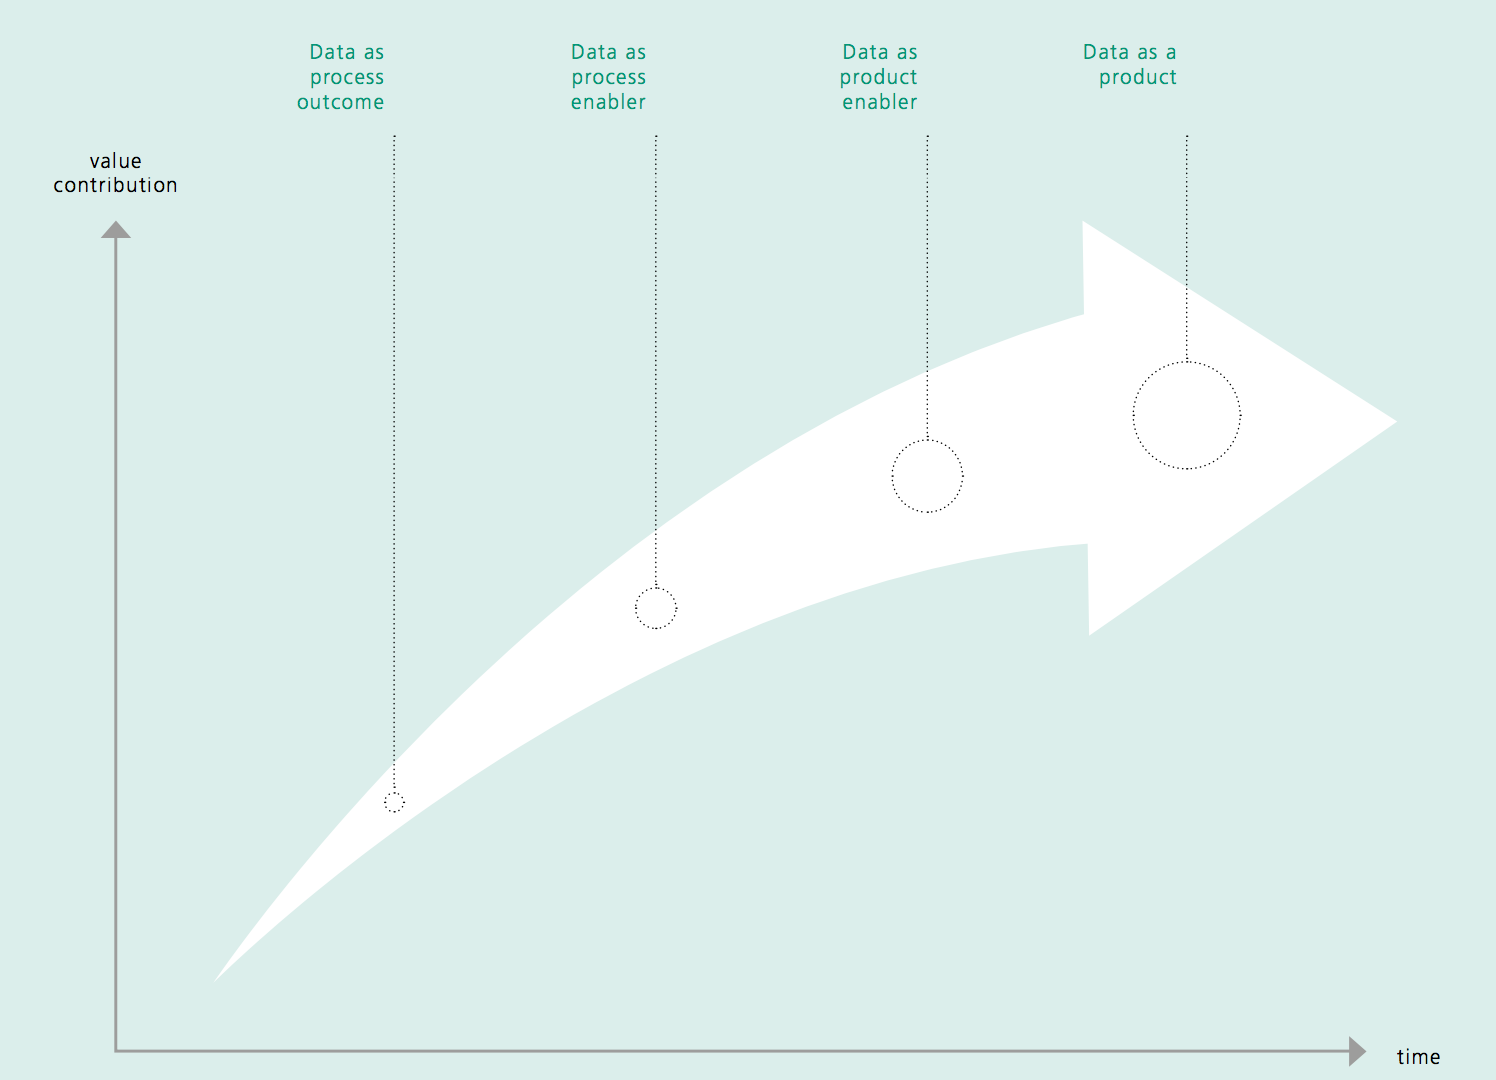
\includegraphics[width=\paperwidth]{images/data}}
\end{center}
%source: https://www.fraunhofer.de/content/dam/zv/en/fields-of-research/industrial-data-space/whitepaper-industrial-data-space-eng.pdf




%data as the result of a process: 
%..


%questions: 
%format of the data, 



%This thesis studies a single board producting machine, cardboard machine 5, that was chosen due to its production problems in (perälaatikon saostumat), (kuivausrummun mällit) and issues with a length-cutter. 


%The current utilization rate of cardboard machine 5 is approximately 80\%, due to the allocation of maintenance schedules, perälaatikon saostuminen, and problems in the length cutter. This thesis aims to identify how to improve the utilization rate of cardboard machine 5 by improving reliability in the components. 



%Maintenance, operations and design data from components of the machine are put into a common cross-enterprise data bazaar. 




%Cross-enterprise data




%Platform:
Marketplace:


\cite{Aijan paperi} Centralized data marketplace:
platform operator provides facilitation services through technical platform

"centralized design can only work as long as its facilitation services result in it being preferable to users compared to repeated bilateral exchanges in terms of cost, reach of suppliers, speed, and so on"

Decentralized data marketplace: structural elements no longer offered by the centralized platform, but executed by data participants.


exhaust data: created as a by-product of other activities such as socializing, rather than specifically for analytical purpose

\cite{schomm2013marketplaces} marketplaces for trading data with varying licensing models




%Kartonkikone 5 valittiin, koska siinä oli tuotanto-ongelmia:
%1 Perälaatikon saostumat -> kuivausrummun mällit
%2 Taru-projektin jäljiltä logistiikan vetäminen, pituusleikkurin jälkeinen homma
%3 




%Production line data from the IT systems of three companies into a shared information operations centre

%A subset of the data is made open for R&D partners, such as start-ups, researchers and students

%Start-up potentials:
%-Data acquisition, data integration and management, data analytics, applications

%Goals:
%-Käyttövarmuuden parantaminen
%-Laitteiden elinkaaren optimointi 
%-Seisokkien keston ja laadun parannukset

%Shared benefits across production life-cycle in
%-Engineering
%-Operations
%-Maintenance

%Key characteristics of the solution
%-Real-time data
%-Mobile & remote operations
%-Predictive actions
%-Increased automation

%Mitä dataa yhteiseen pilveen?

%Laitetiedot (SAP)
%-Toimintopaikkahierarkia
%-Laiterakenne

%Laitteen historiatiedot (SAP + Seitti)
%-Asennustiedot
%-Käyttöönottotiedot
%-Häiriötiedot
%-Huolto- ja korjaustoimenpiteet

%Toimintopaikan prosessitiedot (Impi)
%-Säätöpiirin asetusarvo
%-Säätöpiirin ohjausarvo
%-Säätöpiirin mittausarvo

%-Literature review: minkä teeman lähteitä? cross-enterprise data? Innovation?
%Operations management, Maintenance operations management, Teollisuustaloudellinen näkökunta

%-> uusi ilmiö, Teollinen internet -teema. kulminoituu ohjelmistojen tulemiseksi osaksi teollisuutta. mitä älykkyys tarkoittaa?

%Ohjelmistobisnes, softapuoli.

%kolmas näkökulma: analytiikka, mitä datasta saa irti. 





%laitteiden luotettavuuden parannus -> tuotantotehokkuuden lisäys



%lopputulos: klassifiointi / vaatimusmäärittely datan jakamiselle




%Miten synnyttää olosuhteet jossa yritykset voivat jakaa tietoa keskenään?
%-Minkälainen settingi pitäisi olla jos kannattavaa? Monta yritystä, kilpailijoita mukana?
%Tämänlaisia tavoitteita, näin ne täyttyvät ja ei

%Tutkimuscase: yritykset ei ajattele että tilanne on liiketoimintacase, ja motivaatio on se että tutkitaan jotain keinotekoista











%RQ1: In this business case, what kind of data governance and cross-licensing model are needed to create new business from cross-enterprise data?




%RQ1: Under which cross-licensing models and other commercial conditions should the cross-enterprise data sharing be governed?



%This research question is answered by first identifying which data governacne principles change and how, when instead of a single company a network of companies is considered.
%Data governance, licensing, ..


%RQ2: What other operative innovations in this production environment are enabled (mahdollistaa) by sharing the data? 
%(Jos dataa olisi paremmin saatavilla, sillä olisi arvoa uusien innovaatioiden avulla olisi jo löydös)
%(Kaikilla yrityksillä datasta omat mielenkiinnot)





%Miten data governancen käytännöt muuttuvat kun tarkastellaan yhden yrityksen sijaan usean yrityksen verkkoa?

%What enables new business from cross-enterprise data?





%RQ1: How well can required maintenance be predicted from data collected from the components of cardboard machine 5?  
%RQ1: What added value can vendors bring into the operations of cardboard machine 5? 
%TODO:! Operatiivisen ja maintenance-datan yhdistäminen on jo haastavaa
%Miten dataa yhdistämällä voidaan tuoda lisäarvoa? Mitä lisädataa/arvoa voi metso tuoda?
%Voiko valmet, metso ja muut tuoda jotain lisää, mitä stora enso ja valmet eivät vielä tiedä? benchmarkkeja muista käyttökohteista? domain-osaamista?

%1. Kuinka hyvin koneista kerättävän datan avulla voidaan ennakoida tarvittavat huoltotoimenpiteet?
%jokin rajaus koneisini
%datamallit

%RQ2: How should the collected data be governed?

%This research question aims to identify how the data from three sources, engineering, operations and maintenance, should be governed. To answer the research question, key members from all of the organizations providing data are interviewed. In addition to the qualitative interviews, quantitative questionnaires are sent to 


%Kuka omistaa datan? Kuka omistaa datasta tehdyn mallin?

%2. How should the data be governed?
%	-Engineering, Operations, Maintenance -> kolme datalähdettä integroidaan? Engineering-tietoa ei ole SE:llä juuri käytettävissä
%
%-Haastattelut: ABB, Stora Enso, Metso, Efora, Valmet: mitä dataa? miten kokee hyötyvänsä tästä? miten omistus teidän mielestä mahdollista? ovatko valmiita luovuttamaan? Onko mahdollista rakentaa osuuskunta? -> jokainen tuo oman datansa, hyötyä jaetaan.  
%-Haastattelurungon tueksi kyselylomake, jonka voi lähettää laajemmalle porukalle. 



%3. Mitä muita _operatiivisia innovaatioita_ (tässä tuotantoympäristössä) data mahdollistaa? <- laitetoimittajille todella hyvä mahdollisuus, pystyy lisäämään omaa palvelumyyntiä maailmalla. SE saattaa pystyä optimoimaan energiakulutusta, kartongin laatua}


\section{Structure of the Thesis}
\label{section:structure} 

This thesis is structured as follows. In the third chapter, the relevant literature in operations management, maintenance operations management, shared enterprise data and industrial internet are studied to both educate the reader on the subject and to position this study in the field.


